\section{Offline results: how many validator calls can each signal skip?}\label{sec:results}

\subsection{Path planning}
Table~\ref{tab:skip-fsm} reports the share of validator calls skipped on the fresh certification set. Observable
features alone skip 16--85\% of calls depending on the model, with the failure bound among unchecked accepts
certified for three models. Adding internal signals increases the share of skipped calls for four of the five models
(Fig.~\ref{fig:delta}): by 14.0 points [12.4, 15.5] for Qwen2.5-3B, 15.0 [13.2, 16.9] for Llama-3.2-3B and 6.2 [4.8,
7.5] for SmolLM2 with the full combination, and by 5.1 points [3.7, 6.6] for Qwen2.5-1.5B with grounding alone. For
Llama-3.2-3B, region-based grounding alone carries the whole gain (+15.5 [13.8, 17.3]), and most of these screens
remain certified. Qwen2.5-7B is the exception: its observable screen (15.7\% skipped, certified) is not improved by
internal signals. Internal signals alone skip fewer calls than observables for every model, and token confidence is
the weakest signal throughout.

\begin{table*}[t]
\centering
\small
\caption{FSM: share of validator calls skipped (\%) per signal on the fresh certification set (tolerance $X=10\%$). Bold: failure rate among unchecked accepts certified $\le 10\%$ (one-sided Clopper--Pearson, Bonferroni over signals). $^{+}$/$^{-}$: significantly more/fewer calls skipped than observables (paired bootstrap 95\% CI).}
\label{tab:skip-fsm}
\begin{tabular}{lrrrrr}
\toprule
Signal & Qwen-1.5B & Qwen-3B & Qwen-7B & Llama-3B & SmolLM-1.7B \\
\midrule
Observables & \textbf{40} & \textbf{21} & \textbf{16} & 43 & 85 \\
\midrule
Obs. + grounding & \textbf{46}$^{+}$ & \textbf{21} & 22$^{+}$ & \textbf{59}$^{+}$ & 85 \\
Obs. + all internals & \textbf{37}$^{-}$ & \textbf{32}$^{+}$ & 15 & \textbf{47}$^{+}$ & 79$^{-}$ \\
Obs. + internals + grounding & \textbf{40} & \textbf{34}$^{+}$ & \textbf{15} & \textbf{58}$^{+}$ & 91$^{+}$ \\
\midrule
Region grounding & \textbf{31}$^{-}$ & \textbf{14}$^{-}$ & \textbf{3}$^{-}$ & \textbf{31}$^{-}$ & 80$^{-}$ \\
Attention (regions) & \textbf{35}$^{-}$ & \textbf{21} & 13$^{-}$ & 17$^{-}$ & 75$^{-}$ \\
Hidden states & 22$^{-}$ & \textbf{24}$^{+}$ & 10$^{-}$ & 27$^{-}$ & 74$^{-}$ \\
All internals & \textbf{25}$^{-}$ & \textbf{25}$^{+}$ & \textbf{9}$^{-}$ & \textbf{31}$^{-}$ & 76$^{-}$ \\
All internals + grounding & \textbf{38}$^{-}$ & \textbf{23}$^{+}$ & \textbf{11}$^{-}$ & \textbf{36}$^{-}$ & 79$^{-}$ \\
Token confidence & 13$^{-}$ & 18$^{-}$ & 0$^{-}$ & 14$^{-}$ & 56$^{-}$ \\
\bottomrule
\end{tabular}
\end{table*}


\subsection{CSTR fault recovery}
In the CSTR (Table~\ref{tab:skip-cstr}), observables skip 41--86\% of calls. The picture for internal signals is
different from path planning. They add significantly for three of five models, each in a different way. For
SmolLM2, both the full combination (+4.8 [1.4, 8.3]) and grounding alone (+3.8 [1.4, 6.2]) skip more calls. For
Llama-3.2-3B, adding internals does not change the share skipped but halves the good proposals rejected unchecked
(16 to 8 of 79, difference $-8$ [$-15$, $-2$]). For Qwen2.5-3B, internals make unchecked accepts possible at all under
the bound-based rule (exploratory). For Qwen2.5-1.5B and Qwen2.5-7B, observables are as good as or better than any
combination. Internals alone skip 10--53\% of calls, almost entirely by rejecting clearly failing proposals; the
all-internals screen executes at most one failing proposal unchecked for any model, although single internal signals
can be less safe (hidden states alone for SmolLM2: 9 failing of 65 accepted).

No CSTR screen is certified at $X=10\%$. This is the power limit stated in advance: with 500 certification episodes
and accept sets of 35--130 proposals, the Bonferroni-corrected bound cannot fall below 10\% even with few failures.
The observed failure rates among unchecked accepts were 4--12\% for the observable screens that accepted any
proposal.

\begin{table*}[t]
\centering
\small
\caption{CSTR: share of validator calls skipped (\%) per signal on the certification partition ($X=10\%$); notation as in Table~\ref{tab:skip-fsm}. $^\dagger$Qwen-3B: exploratory re-analysis under the bound-based rule (its sealed sets had been used once before the rule change).}
\label{tab:skip-cstr}
\begin{tabular}{lrrrrr}
\toprule
Signal & Qwen-1.5B & Qwen-3B$^\dagger$ & Qwen-7B & Llama-3B & SmolLM-1.7B \\
\midrule
Observables & 63 & 41 & 86 & 71 & 61 \\
\midrule
Obs. + grounding & 60$^{-}$ & 39 & 86 & 75$^{+}$ & 65$^{+}$ \\
Obs. + all internals & 61 & 51 & 83 & 72 & 66$^{+}$ \\
Obs. + internals + grounding & 61 & 50 & 80$^{-}$ & 74 & 66$^{+}$ \\
\midrule
Region grounding & 27$^{-}$ & 10 & 47$^{-}$ & 38$^{-}$ & 24$^{-}$ \\
Attention (regions) & 30$^{-}$ & 15 & 49$^{-}$ & 48$^{-}$ & 31$^{-}$ \\
Hidden states & 29$^{-}$ & 13 & 50$^{-}$ & 48$^{-}$ & 45$^{-}$ \\
All internals & 29$^{-}$ & 15 & 47$^{-}$ & 53$^{-}$ & 40$^{-}$ \\
All internals + grounding & 28$^{-}$ & 12 & 48$^{-}$ & 53$^{-}$ & 41$^{-}$ \\
Token confidence & 4$^{-}$ & 0 & 17$^{-}$ & 34$^{-}$ & 22$^{-}$ \\
\bottomrule
\end{tabular}
\end{table*}


\begin{figure}[t]
\centering
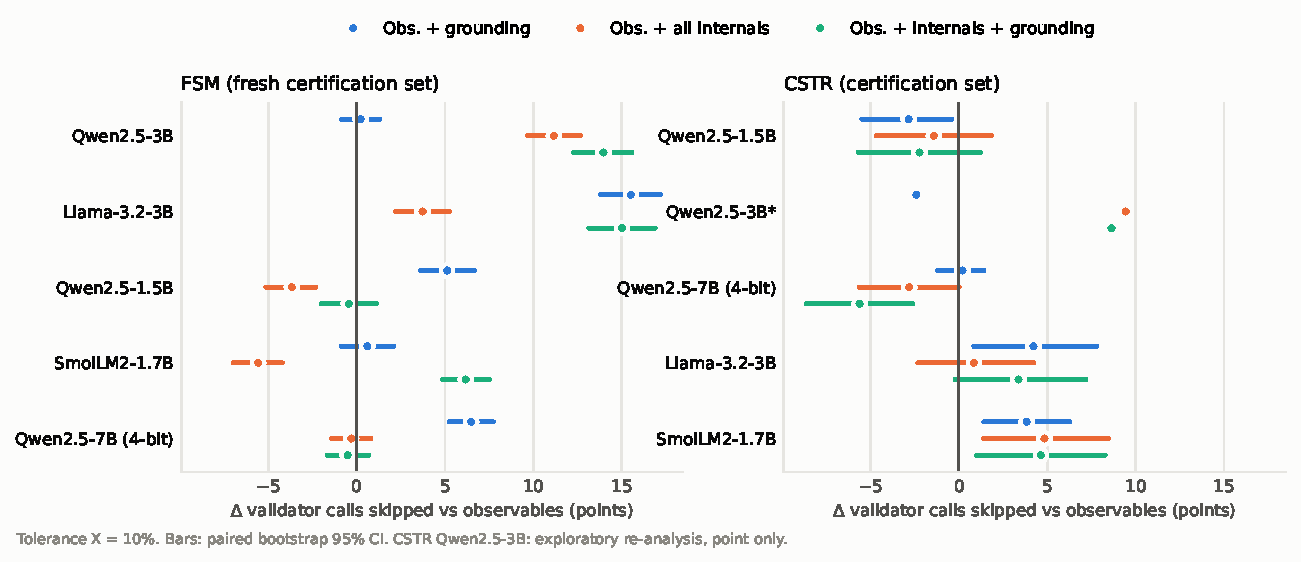
\includegraphics[width=\textwidth]{figures/delta_vs_observables.pdf}
\caption{Change in validator calls skipped relative to the observable screen when grounding, all internal signals,
or both are added (tolerance $X=10\%$, paired bootstrap 95\% CI). Left: path planning, fresh certification set.
Right: CSTR, certification partition.}
\label{fig:delta}
\end{figure}

\subsection{Why internals help in one domain and not the other}
Table~\ref{tab:mechanism} tests the mechanism behind region-based grounding directly: does low attention on the
deciding prompt region predict a failing answer? In path planning it does, strongly, for all five models (AUROC
0.75--0.88). At the level of individual steps, an illegal step receives markedly less attention on the source node's
adjacency line than a legal one (AUROC 0.64--0.81 for the four models analysed at step level). Path-planning failures
are retrieval failures: the information that decides the step is in the prompt, and the model did not consult it.

In the CSTR the signal is weak or absent for three models (0.48--0.52) and moderate for the two smallest (0.66 for
SmolLM2, 0.72 for Qwen2.5-1.5B). A pre-registered test for Qwen2.5-3B makes the contrast explicit. Proposals that
raise the feed while the cooling is saturated and the reactor is hot, a move the physics in the prompt rules out,
receive slightly \emph{more} attention on the physics section than other proposals (AUROC 0.31 for the predicted
direction). The model reads the relevant physics and still reasons to the wrong action. Attention grounding detects
the first kind of failure, not the second, which is why its value is domain dependent. This is consistent with the
view that attention is useful as a predictive signal without being a full explanation of model behaviour
\citep{jain2019attention,wiegreffe2019attention}.

\begin{table}[t]
\centering
\small
\caption{Does low attention on the prompt region that decides the answer predict failure? AUROC of the negative minimum grounding share for answer failure (train + development data; 0.5 = no signal).}
\label{tab:mechanism}
\begin{tabular}{lrr}
\toprule
Model & FSM & CSTR \\
\midrule
Qwen-1.5B & 0.84 & 0.72 \\
Qwen-3B & 0.75 & 0.50 \\
Qwen-7B & 0.72 & 0.48 \\
Llama-3B & 0.84 & 0.52 \\
SmolLM-1.7B & 0.88 & 0.66 \\
\bottomrule
\end{tabular}
\end{table}


\subsection{Robustness to plant and fault shift}
A screen is only useful if it remains valid when the plant population changes. In a pre-registered shift analysis
(Table~\ref{tab:shift}) we fitted probes on one part of the plant and fault space and evaluated them on another,
without recalibration: low to high nominal feed rate (visible in the prompt), low to high heat-transfer coefficient
(not visible), and each fault family held out in turn. All signals degrade under the feed and fault-family shifts, by
0.04--0.28 AUROC for the observable screen, whereas the cooling shift is nearly harmless. Contrary to our
pre-registered expectation, internal signals did not degrade less than observables, and adding them made unchecked
accepts \emph{less} safe on unseen fault types for one model. An earlier, larger shift (one training plant to a varied
population, under a different prompt) had favoured internal signals; we report both and conclude that the screens
must be recalibrated when the plant or fault population changes.

\begin{table}[t]
\centering
\small
\caption{AUROC for failure on the target part of each pre-registered shift (probes fitted on the source part only). Control: random split of the same size.}
\label{tab:shift}
\begin{tabular}{llrrrr}
\toprule
Model & Signal & Control & Feed & Cooling & Fault family \\
\midrule
Qwen-1.5B & Observables & 0.93 & 0.70 & 0.91 & 0.72 \\
 & Obs. + all internals & 0.92 & 0.72 & 0.90 & 0.74 \\
 & All internals & 0.80 & 0.64 & 0.79 & 0.66 \\
 & Token confidence & 0.65 & 0.54 & 0.63 & 0.50 \\
\midrule
Qwen-3B & Observables & 0.87 & 0.73 & 0.86 & 0.80 \\
 & Obs. + all internals & 0.85 & 0.74 & 0.85 & 0.74 \\
 & All internals & 0.71 & 0.60 & 0.72 & 0.62 \\
 & Token confidence & 0.57 & 0.48 & 0.55 & 0.50 \\
\midrule
Qwen-7B & Observables & 0.93 & 0.66 & 0.92 & 0.77 \\
 & Obs. + all internals & 0.92 & 0.65 & 0.91 & 0.71 \\
 & All internals & 0.80 & 0.52 & 0.77 & 0.55 \\
 & Token confidence & 0.68 & 0.47 & 0.66 & 0.54 \\
\midrule
Llama-3B & Observables & 0.90 & 0.86 & 0.91 & 0.80 \\
 & Obs. + all internals & 0.92 & 0.91 & 0.93 & 0.82 \\
 & All internals & 0.84 & 0.83 & 0.86 & 0.71 \\
 & Token confidence & 0.63 & 0.57 & 0.66 & 0.57 \\
\bottomrule
\end{tabular}
\end{table}

